
\section{Related Work}
\setcitestyle{authoryear}
\cite{ntk} showed the NTK to be the central quantity in the study of generalisation properties of infinite width DNNs. \cite{jacot2019freeze} identify two regimes that occur at initialisation in fully connected DNNs as the width increases to infinity namely i) \emph{freeze:} here, the (scaled) NTK converges to a constant and hence leads to slow training,  and  ii) \emph{chaos:} here, the NTK converges to Kronecker delta and hence hurts generalisation. \cite{jacot2019freeze} also suggest that for good generalisation it is important to operate the DNNs at the edge of the freeze and the chaos regimes. \cite{arora2019exact} proposed pure kernel method based on the infinite width CNTK (NTK of convolutional neural network) and showed that it out performed state-of-the-art kernel methods by $10\%$. \cite{arora2019exact} also noted a performance gain (about $5-6\%$) of the CNNs over the CNTK.  However, it was also noted by \cite{arora2019exact,lee2019wide} that random NTFs obtained from finite width neural networks do not perform as well as their limiting infinite width counterparts. 
\cite{arora,cao2019generalization} provided generalisation bounds with the NTK norm. \cite{dudnn} use the NTK to show that over-parameterised DNNs trained by gradient descent achieve zero training error. \cite{dudln,shamir,ganguli} studied deep linear networks. Since deep linear networks are special cases of deep gated networks, \Cref{th:main} of our paper also provides an expression for the NTK at initialisation of deep linear networks. To see this, in the case of deep linear networks, all the gates are always $1$ for all input examples, and $\Lambda_{\Theta}$ will be a matrix whose entries will be $w^{(d-1)}$.

The results in our paper are complementary to the prior NTF/NTK based works, in that, the NPK and NPFs are zeroth order kernel and features respectively. In contrast, the NTF is the gradient of the network output with respect to the weights of the network and hence the NTF/NTK are essentially first order quantities. The fixed NPF regime is different from the NTK regime and the freeze/chaos regimes studied in prior works, in that, in the fixed NPF setting the gates are controlled by a separate feature network.

Gated linearity was studied recently by \cite{sss}, where single layered gated networks were considered. In terms of the work in our paper, \cite{sss} consider the fixed NPF setting with random NPFs of a single layer network. In contrast to the work by \cite{sss}, in this paper we considered DGN of depth $d$, and we also showed (using the DNPFL setting) that by gradient descent on the parameters of the feature and the value network we can learn the NPFs leading to better generalisation than learning with the fixed random NPFs. We believe that handling of depth $d$ networks, identification and the use of novel quantities namely NPFs, NPK and, the role of NPF learning in generalisation amount to significant progress in comparison to \cite{sss}. 

The role of gates was also empirically studied by \cite{srivastava2014understanding}, where the active sub-networks are called as \emph{locally competetive} networks. They encode the active subnetwork information in a sub-mask which is bit string that encodes the $0/1$ state of the all the gates. The sub-masks were then visualised using t-SNE. The visualisation showed that the ``subnetworks active for examples of the same class are much more similar to each other compared to the ones activated for the examples of different classes''. \cite{balestriero2018spline} show the connection between $\max$-affine linearity and DNN with ReLU activations. \cite{neyshabur2015path} used the notion of paths to define a \emph{path-norm} based gradient descent procedure. 
\section{Conclusion}
\begin{comment}
Optimisation and generalisation of DNNs has been an important question in machine learning. Prior works have considered the \emph{neural tangent features} (NTF) and an associated \emph{neural tangent kernel} (NTK), which are quantities based on the first-order gradient information.  In this paper, we looked at fully connected DNNs with ReLU activations, and for such networks, we defined a novel feature namely the \emph{neural path feature} (NPF) and an associated \emph{neural path kernel} , which are \emph{zeroth-order} quantities. The NPFs are based on the information in the gates of a DNN, and hence the NPFs change as the network is trained. We theoretically showed that NPK can be used to understand the optimisation and generalisation for models trained with fixed NPFs. We showed in the experiments that in standard DNNs with ReLU activations, NPFs are learnt during training, and such NPF learning is key for generalisation performance. We also showed via experiments that deep gated networks, where NPFs are learned in a decoupled manner also generalise well. 

A possible future direction is to understand the role of depth and width in NPF learning, and the role of NPF in generalisation. The deep gated network might be useful in this effort, since the NPFs learning is decoupled and is perhaps amenable to analysis in comparison the standard DNNs.
\end{comment}
In this paper, we studied the role of active sub-networks in deep learning by encoding the gates in the neural path features. We showed that the neural path features are learnt during training and such learning is key for generalisation. In our experiments, we observed that almost all information of a trained DNN is stored in the neural path features. We conclude by saying that \emph{understanding deep learning requires understanding neural path feature learning}. %The deep gated network whose gates are decoupled is perhaps an easier starting point to analyse neural path feature learning. 
%A possible future direction is to understand the role of depth and width in NPF learning, and the role of NPF in generalisation.
\begin{comment}
In this paper, we considered the problem of optimisation and generalisation in DNNs with ReLU activations. Throughout the paper, we exploited the special property of the ReLU activation, in that, i output of a ReLU activation be expressed as a product of its pre-activation input and its gating value which is $1/0$ based on whether or not the pre-activation is positive or negative. To analyse such networks, we  introduced the `path-view': a path starts from the input passes through one weight and one hidden nodes per layer and finally ends in the output, and the output of a network is seen as a cumulative combination of the contributions from various paths. The computation in each path was further divided into those happening in the weights, and those happening in the gates. This enabled us to express the output of such DNNs as an inner product of neural path feature (for a path, its feature is the product of gates it encounters from input to output)  and neural path value (for a path, its value is the product of weights it encounters from input to output). The neural path feature (NPF) of a given input is completely dictated by the gating pattern, i.e., the \emph{on/off} status of the gates in the network for that input. Due to the \emph{on/off} nature of the gates, their change to infinitesimal change in the network parameters is $0$, i.e., the gradient of the NPFs with respect to the network weights is $0$. However, in practice the NPFs change during training. By considering a soft-ReLU activation, which served as a `differentiable' substitute for the ReLU activation, we could capture the feature gradient, i.e., the gradient of the NPFs with respect to the network weights. This enabled us to write down the gradient descent dynamics that incorporated NPF learning. We presented the following interesting results:

$1.$ In the fixed NPF regime, wherein, the NPFs are held constant through training, the optimisation and generalisation depends on the associated neural path kernel.

$2.$ 
\end{comment}


\setcitestyle{numbers}
\bibliographystyle{plainnat}
\bibliography{refs}



\newpage
\begin{center}
{\Large{\textbf{Appendix}}}
\end{center}

\begin{appendix}
\section{Expression for $K^{(d)}$}\label{sec:kd}
The $K^{(d)}$ matrix is computed by the recursion in \eqref{eq:ntkold}.
\begin{align}\label{eq:ntkold}
&\tilde{K}^{(1)}(s,s')=\Sigma^{(1)}(s,s')=\Sigma(s,s'), M^{(l)}_{ss'}=\left[\begin{matrix}\Sigma^{(l)}(s,s) & \Sigma^{(l)}(s,s')\\ \Sigma^{(l)}(s',s) & \Sigma^{(l)}(s',s')\end{matrix}\right]\in \R^2,\nn\\
&\Sigma^{(l+1)}(s,s')= 2\cdot\mathbb{E}_{(q,q')\sim N(0,M_{ss'}^{(l)})} \left[\chi(q)\chi(q')\right], \hat{\Sigma}^{(l+1)}(s,s')= 2\cdot\mathbb{E}_{(q,q')\sim N(0,M_{ss'}^{(l)})}\left[\partial\chi(q)\partial{\chi}(q')\right],\nn\\
&\tilde{K}^{(l+1)}=\tilde{K}^{(l)}\odot \hat{\Sigma}^{(l+1)}+\Sigma^{(l+1)}, K^{(d)}=\left(\tilde{K}^{(d)}+\Sigma^{(d)}\right)/2
\end{align}
where $s,s'\in[n]$ are two input examples in the dataset, $\Sigma$ is the data Gram matrix, $\partial{\chi}$ stands for the derivative of the activation function with respect to the pre-activation input, $N(0,M)$ stands for the mean-zero Gaussian distribution with co-variance matrix $M$.

\section{Experimental Setup}\label{sec:expsetup}

\textbf{Dataset:} We used standard datasets namely MNIST and CIFAR-10, with categorical cross entropy loss. We also used a `Binary'-MNIST dataset, which is MNIST with only the two classes corresponding to digits $4$ and $7$, with label $-1$ for digit $4$ and $+1$ for digit $7$. For the `Binary'-MNIST dataset, we used the squared loss.

\textbf{Optimiser and Step-Size:} We used stochastic gradient descent (SGD) and \emph{Adam} as optimisers. In the case of SGD, we tried constant step-sizes in the set $\{0.1,0.01,0.001\}$ and chose the best. In the case of Adam the we used a constant step size of $3e^{-4}$. In both cases, we used batch size to be $32$.


\textbf{Network Architecture:}  

$1.$ We used a fully connected (FC) DNN with $(w=128,d=5)$ for MNIST. 

$2.$ To train CIFAR-10, we used a \emph{Vanilla} CNN architecture denoted by VCONV and a CNN architecture with \emph{global-average-pooling} denoted by GCONV. VCONV is an architecture without pooling, residual connections, dropout or batch-normalisations, and is given by: input layer is $(32, 32, 3)$, followed by convolution layers with a stride of $(3, 3)$ and channels $64$, $64$, $128$, $128$ followed by a flattening to layer with $256$ hidden units, followed by a fully connected layer with $256$ units, and finally a  $10$ width soft-max layer to produce the final predictions. GCONV is same as VCONV with a \emph{global-average-pooling} (GAP) layer at the boundary between the convolutional and fully connected layers.

\textbf{Gating:} 

$1.$ For both FRNPF, and FLNPF, we let $\chi^\text{F}=\chi_r$, and $G_{x,t}(l)= \gamma_{r}\left(q^\text{F}_{x,t}(l)\right)$.

$2.$ In the case, DNPFL, we let $\chi^\text{F}=\chi_r$, and $G_{x,t}(l)= \gamma_{sr}\left(q^\text{F}_{x,t}(l)\right)$. Here $\gamma_{sr}(q)=\frac{1}{(1+\exp(-\beta \cdot q))}$ is a \emph{soft-ReLU} gate which takes values in $(0,1)$. In our experiments we used $\beta=8$. The use of soft-ReLU makes it straightforward for the feature gradients to flow via the gating network.

\textbf{Initialisation:} In the case of FRNPF, we considered two possible initialisations namely i) \emph{independent initialisation} (II), i.e., $\Tg_0$ and $\Tv_0$ are statistically independent, and ii) \emph{dependent initialisation} (DI), i.e., $\Tg_0=\Tv_0$, a case which mimics the NPFs and NPVs of a standard DNN with ReLU activations. In the case of FLNPF, $\Tg_0=\bar{\Theta}$, where $\bar{\Theta}$ is the parameter of a pre-trained (at various stages of training) DNN with ReLU activations. 

\textbf{Epochs:} All the models were trained close to $100\%$ training accuracy. All the models took less than $100$ epochs to train. 

\textbf{Reported Values:} In order to obtain the values in \Cref{tb:npfs}, and in the left most plot of \Cref{fig:dynamics} we used $5$ runs. In each run, we took the best generalisation performance obtained in that run and then averaged the same over $5$ runs.


\section{Applying \Cref{th:main} In Finite Width Case}
%The objective of \Cref{def:gateinfo} was to measure the information stored in the gates of a DNN by storing them in the feature network of a DGN and training the value network.  
In this section, we describe the technical step in applying \Cref{th:main} which requires $w\ra\infty$ to measure the information in the gates of a DNN  with finite width as per \Cref{def:gateinfo}. Since we are training only the value network in the FPNP mode of the DGN, it is possible to let the width of the value network alone go to $\infty$, while keeping the width of the feature network (which stores the fixed NPFs) finite. This is easily achieved by multiplying the width by a positive integer $m\in\Z_{+}$, and \emph{padding} the gates `$m$' times.
\begin{definition}
Define DGN${}^{(m)}$ to be the DGN whose feature network is of width $w$ and depth $d$, and whose value network  is a fully connected network of width $mw$ and depth $d$. The $mw(d-1)$ gating values are obtained by `padding' the $w(d-1)$gating values of the width `$w$', depth `$d$' feature network `$m$' times (see \Cref{fig:dgnpad}, \Cref{tb:dgnpad}). 
\end{definition}

\FloatBarrier
\begin{figure}[!h]
\centering
%\resizebox{\columnwidth}{\textheight}{
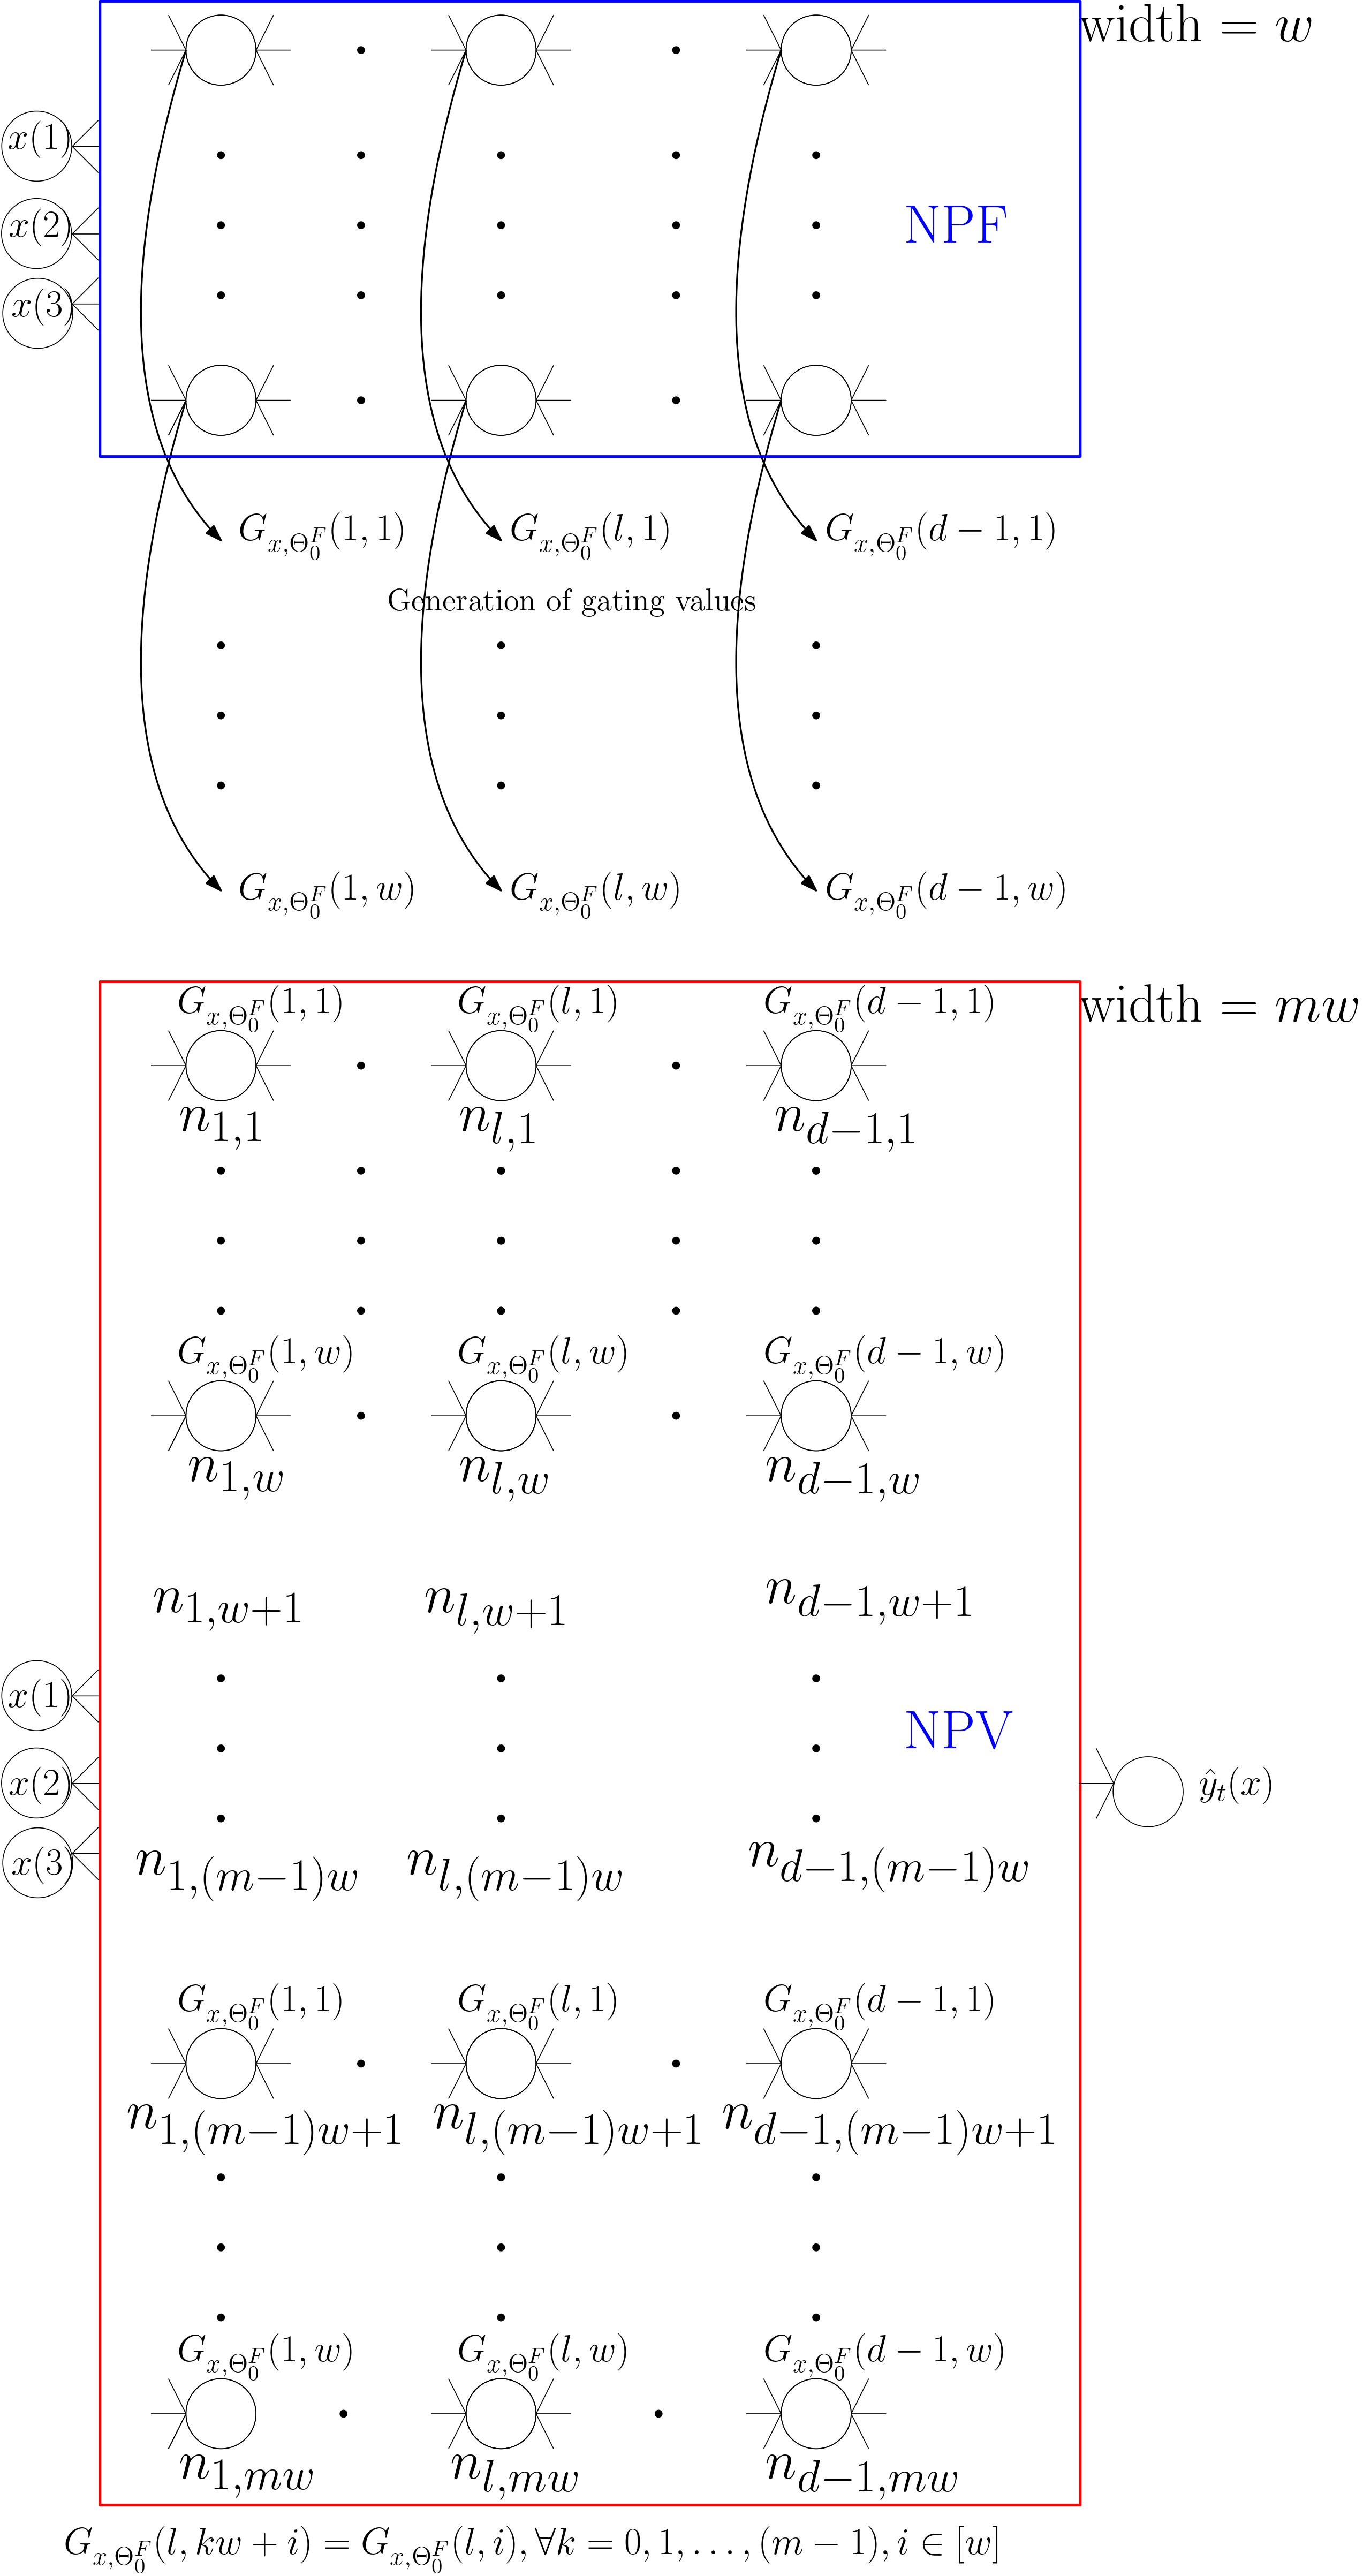
\includegraphics[scale=0.1]{figs/dgn-infty-flipped.png}
%}
\caption{DGN${}^{(m)}$ where the value network is of width $mw$ and depth $d$. The gates are derived by padding the gating values obtained from the feature network `$m$' times, i.e., $ G_{x,t}(l,kw+i)=G_{x,t}(l,i),\forall k=0,1,\ldots,m-1, i\in[w]$.}
\label{fig:dgnpad}
\end{figure}

\begin{table}
\centering
\begin{tabular}{|l|l|l|}\hline
Layer& Feature Network (NPF)& Value Network (NPV)\\
Input & $z^{\text{F}}_{x,t}(0)=x$ &$z^{\text{V}}_{x,t}(0)=x$ \\
Activation & $q^{\text{F}}_{x,t}(l)={\Tg_t(l)}^\top z^{\text{F}}_{x,t}(l-1)$& $q^{\text{V}}_{x,t}(l)={\Tv_t(l)}^\top z^{\text{V}}_{x,t}(l-1)$\\
Hidden &$z^{\text{F}}_{x,t}(l)=\chi^{\text{F}}\left(q^{\text{F}}_{x,t}(l)\right)$& $z^{\text{V}}_{x,t}(l)=q^{\text{V}}_{x,t}(l)\odot G_{x,t}(l)$ \\
Output & None &$\hat{y}_t(x)={\Tv(d)}^\top z^{\text{V}}_{x,t}(d-1)$\\\hline
\multicolumn{3}{|l|}{Gating Values:\quad$ G_{x,t}(l)= \gamma_{r}\left(q^{\text{F}}_{x,t}(l)\right)\quad$or $G_{x,t}(l)= \gamma_{sr}\left(q^{\text{F}}_{x,t}(l)\right)$}\\\hline
\end{tabular}
\caption{Deep Gated Network with padding. Here the gating values are padded, i.e., $ G_{x,t}(l,kw+i)=G_{x,t}(l,i),\forall k=0,1,\ldots,m-1, i\in[w]$. }
\label{tb:dgnpad}
\end{table}

\textbf{Remark:}  DGN${}^{(m)}$ has a total of $P^{(m)}=(mw)^{(d-1)}d_{in}$ paths. Thus, the NPF and NPV are quantities in $\R^{P^{(m)}}$. In what follows, we denote the NPF matrix of DGN${}^{(m)}$ by $\Phi^{(m)}_{\Tg_0}\in\R^{P^{(m)}\times n}$, and use $H^{(m)}_{\text{FNPF}}=(\Phi^{(m)}_{\Tg_0})^\top \Phi^{(m)}_{\Tg_0}$. 

Before we proceed to state the version of \Cref{th:main} for DGN${}^{(m)}$, we will look at an equivalent definition for $\Lambda_{\Theta}$ (see \Cref{def:lambda}).
\begin{definition}\label{def:equilambda}
For input examples $s, s'\in[n]$ define 

$1.$ $\tau_{\Theta}(s,s',l)\stackrel{def}=\sum_{i=1}^w G_{x_s,\Theta}(l,i)G_{x_{s'},\Theta}(l,i)$ be the number of activations that are ``on'' for both inputs $s,s'\in[n]$ in layer $l\in[d-1]$.

$2.$ $\Lambda_{\Theta}(s,s')\stackrel{def}=\Pi_{l=1}^{d-1}\tau_{\Theta}(s,s',l)$.
\end{definition}



\begin{corollary}[Corollary to \Cref{th:main}] Under \Cref{assmp:main} with $\sigma$ replaced by $\sigma_{(m)}=\sigma/\sqrt{m}$, as $m\ra\infty$, $K_{\Theta^{\text{DGN}^{(m)}}_0}\ra K^{(d)}_{\text{FNPF}} = d\cdot \sigma_{(m)}^{2(d-1)} H^{(m)}_{\text{FNPF}}= d\cdot \sigma^{2(d-1)} H_{\text{FNPF}}$.
\end{corollary}
\begin{proof}
Let $\Lambda^{(m)}_{\text{FNPF}}$ and $\tau^{(m)}_{\text{FNPF}}$ be quantities associated with DGN${}^{(m)}$. We know that  $H^{(m)}_{\text{FNFP}}=\Sigma\odot\Lambda^{(m)}_{\text{FNPF}}$. Dropping the subscript FNPF to avoid notational clutter, we have
\begin{align*}
\left(\sigma/\sqrt{m}\right)^{2(d-1)}\Lambda^{(m)}(s,s')&=\sigma^{2(d-1)}\frac{1}{m^{(d-1)}}\Pi_{l=1}^{d-1}\tau^{(m)}(s,s',l)\\
&=\sigma^{2(d-1)}\frac{1}{m^{(d-1)}}\Pi_{l=1}^{d-1}\left(m \tau(s,s',l)\right)\\
&=\sigma^{2(d-1)}\frac{1}{m^{(d-1)}}m^{(d-1)}\Pi_{l=1}^{d-1} \tau(s,s',l)\\
&=\sigma^{2(d-1)}\Pi_{l=1}^{d-1} \tau(s,s',l)\\
&=\sigma^{2(d-1)}\Lambda(s,s')
\end{align*}
\end{proof}


\section{Proofs of technical results}
Proof of \Cref{prop:basic}
\begin{proof}
We know that $e_t=(e_t(s),s\in[n])\in\R^n$, and $e_t(s)=\hat{y}_{\Theta_t}(x_s)-y(s)$. Now
\begin{align} 
L_{\Theta_t}&=\frac{1}2\sum_{s'=1}^n(\hat{y}_{\Theta_t}-y)^2\nn\\
&=\frac{1}2\sum_{s'=1}^n e_t^2\nn\\
\nabla_{\Theta} L_{\Theta_t}&= \sum_{s'=1}^n\nabla_{\Theta} \hat{y}_{\Theta_t}(x_{s'})e_t(s')\nn\\
\label{eq:above1} \nabla_{\Theta} L_{\Theta_t}&= \sum_{s'=1}^n \psi_{x_{s'},\Theta_t}e_t(s')
\end{align}
For gradient descent, $\dot{\Theta}_t=-\nabla_{\Theta} L_{\Theta_t}$, from \eqref{eq:above1} it follows that 
\begin{align}
\dot{\Theta}_t=-\sum_{s'=1}^n \psi_{x_{s'},\Theta_t}e_t(s')
\end{align}
Now $\dot{e}_t=\dot{\hat{y}}_{\Theta_t}$, and expanding $\dot{\hat{y}}_{\Theta_t}(x_s)$ for some $s\in[n]$, we have:
\begin{align}
\dot{\hat{y}}_{\Theta_t}(x_s)&=\frac{d \hat{y}_{\Theta_t}(x_s)}{d t}\nn\\
&=\sum_{\theta\in\Theta}\frac{d \hat{y}_{\Theta_t}(x_s)}{d \theta}\frac{d \theta_t}{dt},\,\text{by expressing this summation as a dot product we obtain} \nn\\
\dot{\hat{y}}_{\Theta_t}(x_s)&=\ip{\psi_{x_s,\Theta_t},\dot{\Theta}_t}
\end{align}
We now use that fact that $\Theta_t$ is updated by gradient descent
\begin{align}
\dot{\hat{y}}_{\Theta_t}(x_s)&=-\ip{\psi_{x_s,\Theta_t},\sum_{s'=1}^n \psi_{x_{s'},\Theta_t}e_t(s')}\nn\\
&=-\sum_{s'=1}^n K_{\Theta_t}(s,s')e_t(s')
\end{align}
The proof is complete by recalling that $\hat{y}_{\Theta_t}=(\hat{y}_{\Theta_t}(x_s),s\in[n])$, and $\dot{e}_t=\dot{\hat{y}}_{\Theta_t}$.
\end{proof}


Proof of \Cref{prop:zero}
\begin{proof}
Let $x\in\R^{d_{in}}$ be the input to the DNN and $\hat{y}_{\Theta}(x)$ be its output. The output can be written in terms of the final hidden layer output 
\begin{align}
\hat{y}_{\Theta}(x)&={\Theta(d)}^\top z_{x,\Theta}(d-1)\nn\\
&=\sum_{j_{d-1}=1}^w\Theta(d, j_{d-1},1)  z_{x,\Theta}(d-1,j_{d-1})\nn\\
\label{lastlayer}&=\sum_{j_{d-1}=1}^w\Theta(d, j_{d-1},1)  G_{x\Theta}(d-1,j_{d-1}) q_{x,\Theta}(d-1,j_{d-1})
\end{align}
Now $q_{x,\Theta}(d-1,j_{d-1})$ for a fixed $j_{d-1}$ can again be expanded as
\begin{align}
q_{x,\Theta}(d-1,j_{d-1})&= \sum_{j_{d-2}=1}^w \Theta(d, j_{d-2}, j_{d-1}) z_{x,\Theta}(d-2,j_{d-2})\nn\\
\label{onebefore}&=\sum_{j_{d-2}=1}^w \Theta(d-1, j_{d-2}, j_{d-1}) G_{x,\Theta}(d-2,j_{d-2})q_{x,\Theta}(d-2,j_{d-2})
\end{align}
Now plugging in \eqref{onebefore} in the expression in \eqref{lastlayer}, we have
\begin{align}
\hat{y}_{\Theta}(x)&=\sum_{j_{d-1}=1}^w\Theta(d, j_{d-1},1)  G_{x\Theta}(d-1,j_{d-1}) \left(\sum_{j_{d-2}=1}^w \Theta(d-1, j_{d-2}, j_{d-1}) G_{x,\Theta}(d-2,j_{d-2})q_{x,\Theta}(d-2,j_{d-2})\right)\nn\\
&=\sum_{j_{d-1}, j_{d-2}\in[w]} G_{x,\Theta}(d-1,j_{d-1}) G_{x,\Theta}(d-2,j_{d-2}) \Theta(d, j_{d-1},1) \Theta(d-1, j_{d-2}, j_{d-1}) q_{x,\Theta}(d-2,j_{d-2})\nn\\
\end{align}
By expanding $q$'s for all the previous layers till the input layer we have
\begin{align}
\sum_{j_{d}=1, j_{d-1},\ldots,j_{1}\in[w], j\in[d_{in}]} x(j) \Pi_{l=1}^{d-1}G_{x,\Theta}(l,j_{l}) \Pi_{l=1}^{d}\Theta(l, j_{l-1}, j_{l}) \nn
\end{align}
\end{proof}

Proof of \Cref{lm:npk}
\begin{proof}
\begin{align}
\ip{\phi_{x_s,\Theta},\phi_{x_{s'},\Theta}}&=\sum_{p\in[P]}x_s(\I_0(p))x_{s'}(\I_0(p))A_{\Theta}(x_s,p)A_{\Theta}(x_{s'},p)\nn\\
&=\sum_{i=1}^{d_{in}}x_s(i)x_{s'}(i)\Lambda_{\Theta}(s,s')\nn\\
&=\ip{x_s,x_{s'}}\cdot\Lambda_{\Theta}(s,s')
\end{align}
\end{proof}

Proof of \Cref{prop:ntknew}
\begin{proof}
Let $\Psi_{\Theta}=(\psi_{x_s,\Theta},s\in[n])\in\R^{d_{net}\times n}$ be the NTF matrix, then the NTK matrix is given by $K_{\Theta_t}=\Psi^\top_{\Theta_t}\Psi_{\Theta_t}$. Note that, $\hat{y}_{\Theta}(x_s)=\ip{\phi_{x_s,\Theta},v_{\Theta}}=\ip{v_{\Theta},\phi_{x_s,\Theta}}=v^\top_{\Theta}\phi_{x_s,\Theta}$. Now $\psi_{x_{s},\Theta}=\nabla_{\Theta} v_{\Theta}\phi_{x_s,\Theta}$, and hence $\Psi=\nabla_{\Theta} v_{\Theta}\Phi_{\Theta}$. Hence, $K_{\Theta_t}=\Psi^\top_{\Theta_t}\Psi_{\Theta_t}=\Phi^\top_{\Theta}(\nabla_{\Theta} v_{\Theta})^\top (\nabla_{\Theta} v_{\Theta})\Phi_{\Theta}=\Phi^\top_{\Theta}\V_{\Theta}\Phi_{\Theta}$.
\end{proof}

Proof of \Cref{prop:dnnhard}

\begin{proof}
Follows in a similar manner as the proof of \Cref{prop:basic}.
\end{proof}

Proof of {\Cref{prop:condition}}
\begin{proof}
$\rho_{\min}(K_{\Theta})=\underset{\norm{x}_2=1}{\underset{x\in \R^n}\min}x^\top K_{\Theta} x$. Let $x'\in\R^n$ such that $\norm{x'}_2=1$ and $\rho_{\min}(K_{\Theta})={x'}^\top K_{\Theta} x'$. Now, let $y'=\Phi x'$. Then we have, $\rho_{\min}(K_{\Theta})={y'}^\top \V_{\Theta}y'$. Hence $\rho_{\min}(K_{\Theta})\leq \norm{y'}^2_2 \rho_{\max}(\V_{\Theta})$. Now, $\norm{y'}^2_2={x'}^\top \Phi^\top_{\Theta}\Phi_{\Theta}x'\leq \rho_{min}(H_{\Theta})$.
\end{proof}


Proof of \Cref{prop:dgn}

\begin{proof}
Follows in a similar manner as proof of \Cref{prop:basic}.
\end{proof}


\begin{lemma}\label{lm:dot}
Let $\varphi_{p,\Theta}$ be as in \Cref{def:npvgrad}, under Assumption~\ref{assmp:main}, for paths $p,p_1,p_2\in \P, p_1\neq p_2$, at initialisation we have (i) $\E{\ip{\varphi_{p_1,\Tv_0}, \varphi_{p_2,\Tv_0}}}= 0$, (ii) ${\ip{\varphi_{p,\Tv_0}, \varphi_{p,\Tv_0}}}= d\sigma^{2(d-1)}$.
\end{lemma}

\begin{proof}
\begin{align*}
\ip{\varphi_{p_1,\Tv_0}, \varphi_{p_2,\Tv_0}}= \sum_{\tv\in \Tv} \partial_{\tv}v_{\Tv_0}(p_1) \partial_{\tv}v_{\Tv_0}(p_2)
\end{align*}
Let $p\rsa(\cdot)$ denote the fact that path $p$ passes through $(\cdot)$, and let $p\bcancel\rsa(\cdot)$ denote the fact that path $p$ does not pass through $\bcancel\rsa$. Let $\tv\in\Tv$ be any weight such that $p\rsa \tv$, and w.l.o.g let $\tv$ belong to layer $l'\in[d]$. If either $p_1\bcancel{\rsa}\tv$ or $p_2\bcancel{\rsa}\tv$, then it follows that $\partial_{\tv} v_{\Tv_0}(p_1) \partial_{\tv} v_{\Tv_0}(p_2)=0$. In the case when $p_1,p_2\rsa\tv$, we have
\begin{align*}
&\E{\partial_{\tv}v_{\Tv_0}(p_1)\partial_{\tv}v_{\Tv_0}(p_2)}\\
&=\E{\underset{l\neq l'}{\underset{l=1}{\overset{d}{\Pi}}} \Bigg(\Tv_0(l, \I_{l-1}(p_1),\I_{l} (p_1))\Tv_0(l,\I_{l-1} (p_2),\I_{l}(p_2)) \Bigg)}\\
&=\underset{l\neq l'}{\underset{l=1}{\overset{d}{\Pi}}}\E{\Tv_0(l,\I_{l-1}(p_1),\I_{l}(p_1))\Tv_0(l,\I_{l-1}(p_2),\I_{l}(p_2))}
\end{align*}
where the $\E{\cdot}$ moved inside the product because at initialisation the weights (of different layers) are independent of each other.
Since $p_1\neq p_2$, in one of the layers $\tilde{l}\in[d-1],\tilde{l}\neq l'$ they do not pass through the same weight, i.e., $\Tv_0(\tilde{l},\I_{\tilde{l}-1}(p_1),\I_{\tilde{l}}(p_1))$ and $\Tv_0(\tilde{l},\I_{\tilde{l}-1}(p_2),\I_{\tilde{l}}(p_2))$ are distinct weights. Using this fact
\begin{align*}
&\E{\partial_{\tv}v_{\Tv_0}(p_1)\partial_{\tv}v_{\Tv_0}(p_2)}\\
&=\underset{l\neq l',\tilde{l}}{\underset{l=1}{\overset{d}{\Pi}}}\E{\Tv_0(l, \I_{l-1}(p_1),\I_l(p_1))\Tv_0(l,\I_{l-1}(p_2),\I_{l}(p_2))}\\
&=\E{\Tv_0(\tilde{l},\I_{\tilde{l}-1} (p_1),\I_{\tilde{l}}(p_1))}\E{\Tv_0(\tilde{l},\I_{\tilde{l}-1 }(p_2),\I_{\tilde{l}}(p_2))}\\
&=0
\end{align*}

The proof of (ii) is complete by noting that $\sum_{\tv\in\Tv} \partial_{\tv}v_{\Tv_0}(p) \partial_{\tv}v_{\Tv_0}(p)$ has $d$ non-zero terms for a single path $p$ and at initialisation we have 
\begin{align*}
&\partial_{\tv}v_{\Tv_0}(p) \partial_{\tv}v_{\Tv_0}(p) \\
&={\underset{l\neq l'}{\underset{l=1}{\overset{d}{\Pi}}} {\Tv_0}^2(l,\I_{l-1}(p),\I_{l}(p))}\\
&=\sigma^{2(d-1)}
\end{align*}
\end{proof}

\textbf{Detailed version of \Cref{th:main} with proof.}
\begin{theorem}\label{th:mainrefined}
Under \Cref{assmp:main}, and $\frac{4d}{w^2}<1$ it follows that
 \begin{align*}
\E{K_{\Tdgn_0}}&=d\cdot\sigma^{2(d-1)} H_{\text{FNPF}}\\
Var\left[K_{\Tdgn_0}(s,s')\right]&\leq O\left(d^2_{in}\sigma^{4(d-1)}\max\{d^2w^{2(d-2)+1}, d^3w^{2(d-2)}\}\right)
\end{align*}
\end{theorem}

\begin{proof}
We have 
\begin{align*}
\E{K_{\Tdgn_0}}&=\E{\Phi^\top_{\text{FNPF}} \V_{\Tv_0} \Phi_{\text{FNPF}}}\\
&=\E{\Phi^\top_{\text{FNPF}} (\nabla_{\Tv}v_{\Tv_0})^\top (\nabla_{\Tv}v_{\Tv_0}) \Phi_{\text{FNPF}}}\\
&=\Phi^\top_{\text{FNPF}} \E{(\nabla_{\Tv}v_{\Tv_0})^\top (\nabla_{\Tv}v_{\Tv_0})}\Phi_{\text{FNPF}}\\
&\stackrel{(a)}=d\cdot\sigma^{2(d-1)} \Phi^\top_{\text{FNPF}}\Phi_{\text{FNPF}}\\
&=d\cdot\sigma^{2(d-1)} H_{\text{FNPF}}
\end{align*}
where, $(a)$ follows from \Cref{lm:dot}.

We now turn to the variance calculation. The idea is that we expand  $Var\left[K_0(s,s')\right]=\E{K_0(s,s')^2} -\E{K_0(s,s')}^2$ and identify the terms which cancel due to subtraction and then bound the rest of the terms.

\textbf{Notation:} In what follows, we let $K_0$ to denote $K_{\Tdgn_0}$ and drop superscript V from $\Tv_0$, and subscript $\Tv_0$ from $v_{\Tv_0}$. Further, we assume that the weights can be enumerated as $\theta(1),\ldots, \theta(d_{net})$. We also denote $p\rsa (\cdot)$ to denote the fact that path $p$ passes through $(\cdot)$ and $p\bcancel{\rsa}(\cdot)$ to denote the fact that path $p$ does not pass through $(\cdot)$. We use a shortcut notation $A(s,p)$ instead of $A(x_s,p)$. In what follows, we let $x\in\R^{d_{in}\times n}$ to be the data matrix.

 Let $\theta(m),m\in[d_{net}]$ belong to layer $l'(m)$, then 
\begin{align}\label{eq:kexpect} 
&\E{K_0(s,s')}\nn\\
&=\sum_{m=1}^{d_{net}}\E{\left(\sum_{p_1 \in[P]}x(\I_0(p_1),s)A_0(s,p_1)\frac{\partial v_0(p_1)}{\partial \theta(m)}\right)\left(\sum_{p_2\in[P]}x(\I_0(p_2),s)A_0(s',p_2)\frac{\partial v_0(p_2)}{\partial \theta(m)}\right)}\nn\\
&=\sum_{m=1}^{d_{net}}\E{\sum_{p_1,p_2\in[P]}x(\I_0(p_1),s)A_0(s,p_1)\frac{\partial v_0(p_1)}{\partial \theta(m)}x(\I_0(p_2),s')A_0(s',p_2)\frac{\partial v_0(p_2)}{\partial \theta(m)}}\nn\\
&\stackrel{(a)}=\sum_{m=1}^{d_{net}}\underset{p_1,p_2\rsa\theta(m)}{\sum_{p_1,p_2\in[P]}}x(\I_0(p_1),s)A_0(s,p_1)x(\I_0(p_2),s')A_0(s',p_2) \mathbb{E}\Bigg[\underset{l\neq l'(m)}{\underset{l=1}{\overset{d-1}{\Pi}}} \Tb_0(l,\I_{l-1}(p_1),\I_{l}(p_1)) \nn\\&\Tb_0(l,\I_{l-1}(p_2),\I_{l}(p_2))\Bigg]\nn\\
&\stackrel{(b)}=\sum_{m=1}^{d_{net}}\underset{p_1,p_2\rsa\theta(m)}{\sum_{p_1,p_2\in[P]}}x(\I_0(p_1),s)A_0(s,p_1)x(\I_0(p_2),s')A_0(s',p_2) \underset{l\neq l'(m)}{\underset{l=1}{\overset{d-1}{\Pi}}} \mathbb{E}\Bigg[ \Tb_0(l,\I_{l-1}(p_1),\I_{l}(p_1))\nn\\
& \Tb_0(l,\I_{l-1}(p_2),\I_{l}(p_2))\Bigg]
\end{align}
where $(a)$ follows from the fact that for $p\bcancel{\rsa}\theta(m)$, $\frac{\partial v_0(p)}{\partial \theta(m)}=0$, and $(b)$ follows from the fact that at initialisation the layer weights are independent of each other. Note that the right hand side of \eqref{eq:kexpect} only terms with $p_1=p_2$ will survive the expectation.

In the following expression in \eqref{eq:kexpectsquare}, note that only terms of the form $p_1=p_2$ and $p_3=p_4$ are non-zero.

\begin{align*}
&\E{K_0(s,s')}^2=\\
&\Bigg(\sum_{m=1}^{d_{net}}\underset{p_1,p_2\rsa\theta(m)}{\sum_{p_1,p_2\in[P]}}x(\I_0(p_1),s)A_0(s,p_1)x(\I_0(p_2),s')A_0(s',p_2) \underset{l\neq l'(m)}{\underset{l=1}{\overset{d-1}{\Pi}}} \mathbb{E}\Big[\Tb_0(l,\I_{l-1}(p_1),\I_{l}(p_1)) &\\ 
&\Tb_0(l,\I_{l-1}(p_2),\I_{l}(p_2))\Big]\Bigg)\times\\
&\Bigg(\sum_{m'=1}^{d_{net}}\underset{p_3,p_4\rsa\theta(m')}{\sum_{p_3,p_4\in[P]}}x(\I_0(p_3),s)A_0(s,p_3)x(\I_0(p_4),s')A_0(s',p_4) \underset{l\neq l'(m')}{\underset{l=1}{\overset{d-1}{\Pi}}} \mathbb{E}\Big[\Tb_0(l,\I_{l-1}(p_3),\I_{l}(p_3)) &\\
&\Tb_0(l,\I_{l-1}(p_4),\I_{l}(p_4))\Big]\Bigg)\\
\end{align*}
\begin{align}\label{eq:kexpectsquare}
&\E{K_0(s,s')}^2=\nn\\
&\sum_{m,m'=1}^{d_{net}}\underset{p_3,p_4\rsa\theta(m')}{\underset{p_1,p_2\rsa\theta(m)}{\sum_{p_1,p_2,p_3,p_4\in[P]}}}\Bigg[\bigg(x(\I_0(p_1),s)A_0(s,p_1)x(\I_0(p_2),s')A_0(s',p_2)x(\I_0(p_3),s)\nn\\ 
&A_0(s,p_3)x(\I_0(p_4),s')A_0(s',p_4)\bigg)\times \bigg( \underset{l\neq l'(m)} {\underset{l\neq l'(m')}{\underset{l=1}{\overset{d-1}{\Pi}}}} \E{\Tb_0(l,\I_{l-1}(p_1),\I_{l}(p_1)) \Tb_0(l,\I_{l-1}(p_2),\I_{l}(p_2))}\nn\\
&\E{\Tb_0(l,\I_{l-1}(p_3),\I_{l}(p_3)) \Tb_0(l,\I_{l-1}(p_4),\I_{l}(p_4))} \bigg)\times\nn\\
&\bigg( \E{\Tb_0(l,\I_{l'(m')-1}(p_1),\I_{l'(m')}(p_1)) \Tb_0(l,\I_{l'(m')-1}(p_2),\I_{l'(m')}(p_2))}\bigg)\times\nn\\
&\bigg(\E{\Tb_0(l,\I_{l'(m)-1}(p_3),\I_{l'(m)}(p_3)) \Tb_0(l,\I_{l'(m)-1}(p_4),\I_{l'(m)}(p_4))} \bigg)\Bigg]
\end{align}
In the expression in \eqref{eq:ksquareexpect}, paths $p_1,p_2,p_3,p_4$ do not have constraints, and can be distinct.
\begin{align}\label{eq:ksquareexpect}
&\E{K^2_0(s,s')}=\nn\\
&\sum_{m,m'=1}^{d_{net}}\underset{p_3,p_4\rsa\theta(m')}{\underset{p_1,p_2\rsa\theta(m)}{\sum_{p_1,p_2,p_3,p_4\in[P]}}}\Bigg[\bigg(x(\I_0(p_1),s)A_0(s,p_1)x(\I_0(p_2),s')A_0(s',p_2)x(\I_0(p_3),s)\nn\\&
A_0(s,p_3)x(\I_0(p_4),s')A_0(s',p_4)\bigg)\times\bigg( \underset{l\neq l'(m)} {\underset{l\neq l'(m')}{\underset{l=1}{\overset{d-1}{\Pi}}}} \mathbb{E}[\Tb_0(l,\I_{l-1}(p_1),\I_{l}(p_1)) \Tb_0(l,\I_{l-1}(p_2),\I_{l}(p_2))\nn\\&
\Tb_0(l,\I_{l-1}(p_3),\I_{l}(p_3)) \Tb_0(l,\I_{l-1}(p_4),\I_{l}(p_4))] \bigg)\times\nn\\
&\bigg( \E{\Tb_0(l,\I_{l'(m')-1}(p_1),\I_{l'(m')}(p_1)) \Tb_0(l,\I_{l'(m')-1}(p_2),\I_{l'(m')}(p_2))}\bigg)\times\nn\\
&\bigg(\E{\Tb_0(l,\I_{l'(m)-1}(p_3),\I_{l'(m)}(p_3)) \Tb_0(l,\I_{l'(m)-1}(p_4),\I_{l'(m)}(p_4))} \bigg)\Bigg]
\end{align}

We now state the following facts/observations.

$\bullet$ \emph{Fact 1:} Any term that survives the expectation (i.e., does not become $0$) and participates in \eqref{eq:ksquareexpect} is of the form $\sigma^{4(d-1)}\big(x(\I_0(p_1),s)A_0(s,p_1)x(\I_0(p_2),s')A_0(s',p_2)x(\I_0(p_3),s)A_0(s,p_3)x(\I_0(p_4),s')A_0(s',p_4)\big)$, where $p_1,p_2,p_3,p_4$ are free variables. Any term that survives the expectation (i.e., does not become $0$) and participates in participates in \eqref{eq:kexpectsquare} is of the form $\sigma^{4(d-1)}\big(x(\I_0(p_1),s)A_0(s,p_1)x(\I_0(p_2),s')A_0(s',p_2)x(\I_0(p_3),s)A_0(s,p_3)x(\I_0(p_4),s')A_0(s',p_4)\big)$, where $p_1=p_2,p_3=p_4$.

$\bullet$ \emph{Fact 2:} The number of paths through a particular weight $\theta(m)$ in one of the middle layers is $d_{in}w^{d-3}$. The number of paths through a particular weight $\theta(m)$ in the first layer is $w^{d-2}$ . The number of paths through a particular weight $\theta(m)$ in the last layer is $d_{in}w^{d-2}$ .


$\bullet$ \emph{Fact 3:} Let $\P'$ be an arbitrary set of paths constrained to pass through some set of weights. Let $\P''$ be the set of paths obtained by adding an additional constraint that the paths also should pass through a particular weight say $\theta(m)$. Now, if $\theta(m)$ belongs to :

$1.$ a middle layer, then $|\P''|=\frac{|\P'|}{w^2}$.

$2.$ the first layer, then $|\P''|=\frac{|\P'|}{d_{in}w}$.

$3.$  the last layer, then $|\P''|=\frac{|\P'|}{w}$.

$\bullet$ \emph{Fact 4:} For any $p_1,p_2,p_3,p_4$ combination that survives the expectation in \eqref{eq:ksquareexpect} can be written as 

\begin{align*}
&\bigg(x(\I_0(p_1),s)A_0(s,p_1)x(\I_0(p_2),s')A_0(s',p_2)x(\I_0(p_3),s)\\
&A_0(s,p_3)x(\I_0(p_4),s')A_0(s',p_4)\bigg)\times\\
&\bigg( \underset{l\neq l'(m)} {\underset{l\neq l'(m')}{\underset{l=1}{\overset{d-1}{\Pi}}}} \mathbb{E}[\Tb_0(l,\I_{l-1}(p_1),\I_{l}(p_1)) \Tb_0(l,\I_{l-1}(p_2),\I_{l}(p_2))\nn\\
&\Tb_0(l,\I_{l-1}(p_3),\I_{l}(p_3)) \Tb_0(l,\I_{l-1}(p_4),\I_{l}(p_4))] \bigg)\times\nn\\
&\bigg( \E{\Tb_0(l,\I_{l'(m')-1}(p_1),\I_{l'(m')}(p_1)) \Tb_0(l,\I_{l'(m')-1}(p_2),\I_{l'(m')}(p_2))}\bigg)\times\nn\\
&\bigg(\E{\Tb_0(l,\I_{l'(m)-1}(p_3),\I_{l'(m)}(p_3)) \Tb_0(l,\I_{l'(m)-1}(p_4),\I_{l'(m)}(p_4))} \bigg)\nn\\
%&=\\
%&\bigg( \underset{l\neq l'(m)} {\underset{l\neq l'(m')}{\underset{l=1}{\overset{d-1}{\Pi}}}} \Tb^2_0(l,\I_{l-1}(\rho_a),\I_{l}(\rho_a)) \Tb^2_0(l,\I_{l-1}(\rho_b),\I_{l}(\rho_b)) \bigg)\times \bigg( \Tb^2_0(l,\I_{l'(m')-1}(\rho_a),\I_{l'(m')}(\rho_a))\bigg)\nn\\
%&\times \bigg({\Tb^2_0(l,\I_{l'(m)-1}(\rho_b),\I_{l'(m)}(\rho_b))} \bigg),
\end{align*}

where $\rho_a\rsa \theta(m)$ and $\rho_b\rsa \theta(m')$ are what we call as \emph{base} (case) paths. 


$\bullet$ \emph{Fact 5:} For any given base paths $\rho_a$ and $\rho_b$ there could be multiple assignments possible for $p_1,p_2,p_3,p_4$.

$\bullet$ \emph{Fact 6:}  Terms in \eqref{eq:ksquareexpect}, wherein, the base case is generated as $p_1=p_2=\rho_a$ and $p_3=p_4=\rho_b$ (or $p_1=p_2=\rho_b$ and $p_3=p_4=\rho_a$), get cancelled with the corresponding terms in \eqref{eq:kexpectsquare}.

$\bullet$ \emph{Fact 7:}  When the bases paths $\rho_a$ and $\rho_b$ do not intersect (i.e., do not pass through the same weight in any one of the layers), the only possible assignment is $p_1=p_2=\rho_a$ and $p_3=p_4=\rho_b$ (or $p_1=p_2=\rho_b$ and $p_3=p_4=\rho_a$), and such terms are common in \eqref{eq:ksquareexpect} and \eqref{eq:kexpectsquare}, and hence do not show up in the variance term.


$\bullet$ \emph{Fact 7:} Let base paths $\rho_a$ and $\rho_b$ intersect/cross at layer $l_1, \ldots, l_k, k \in [d-1]$, and let $\rho_a=(\rho_a(1),\ldots,\rho_a(k+1))$ where $\rho_a(1)$ is a sub-path string from layer $1$ to $l_1$, and $\rho_a(2)$ is the sub-path string from layer $l_1+1$ to $l_2$ and so on, and $\rho_a(k+1)$ is the sub-path string from layer $l_k+1$ to the output node. Then the set of paths that can occur in $\E{K_0(s,s')^2}$ are of the form:
\begin{enumerate}
\item $p_1=p_2=\rho_a, p_3=p_4=\rho_b$ (or $p_1=p_2=\rho_b, p_3=p_4=\rho_a$) which get cancelled in the $\E{K_0(s,s')}^2$ term.
\item $p_1=\rho_a$, $p_3=\rho_b$, $p_2=(\rho_b(1),\rho_a(2),\rho_a(3),\ldots,\rho_a(k+1))$, $p_4=(\rho_a(1),\rho_b(2),\rho_b(3),\ldots,\rho_b(k+1))$, which are obtained by \emph{splicing} the base paths in various combinations. Note that for such spliced paths $p_1\neq p_2$ and $p_3\neq p_4$ and hence do not occur in the expression for $\E{K_0(s,s')}^2$ in \eqref{eq:kexpectsquare}.
\end{enumerate}


$\bullet$ \emph{Fact 8:} For $k$ crossings of the base paths there are $4^{k+1}$ splicings possible, and those many terms are extra in the $\E{K_0(s,s')^2}$ expression in \eqref{eq:ksquareexpect}, when compared to the $\E{K_0(s,s')}^2$ expression in \eqref{eq:kexpectsquare}. 

\textbf{Upper Bound:} We now enumerate various possible crossings of the base paths, and calculate an upper bound for the magnitude of the contribution of `spliced' terms to the variance term using the \emph{Fact 1} to \emph{Fact 8}. In short, we find an upper bound for the those terms that do not get cancelled in the variance calculation. Further, without loss of generality we drop $x(\I_0(p))$ and $A(\cdot,\cdot)$ terms in this upper calculation.

\textbf{Case $1$:} $k=1$ crossing, in either first or last layer. There are $d_{in}w$ weights in the first layer and $w$ weights in the last layer. The number of base path combinations passing through the first layer is $w^{d-2}\times w^{d-2}$. The number of base path combinations passing through the last layer is ($d_{in}w^{d-2})\times (d_{in}w^{d-2})$.  For each of these cases, $m,m'$ could take $O(d^2)$ possible values. And the multiplication of the weights themselves contribute to $\sigma^{4(d-1)}$.  Splicing of these base paths could be done in $4^2$ ways. Putting them together we have
\begin{align*}
&\sigma^{4(d-1)}\times(w)\times (d^2_{in} \times w^{d-2}\times w^{d-2})\times d^2\times 4^2\\
&+\sigma^{4(d-1)}\times (d_{in}w) \times(w^{d-2}\times w^{d-2}) \times d^2\times  4^2\\
&\leq 32d^2_{in}\sigma^{4(d-1)}d^2 w^{2(d-2)+1}
\end{align*}

\textbf{Case $2$:} $k=1$ crossing, in one of the middle layers. There are $w^2(d-2)$ weights in the middle layers. The number of base path combinations  that pass through a given weight in the middle layers is $(d_{in}w^{d-3})\times(d_{in} w^{d-3})$. For each of these cases, $m,m'$ could take $O(d^2)$ possible values. And the multiplication of the weights themselves contribute to $\sigma^{4(d-1)}$. Splicing of these base paths could be done in $4^2$ ways. Putting them together we have
\begin{align*}
\sigma^{4(d-1)} \times w^2(d-2)\times (d^2_{in}\times w^{d-3}\times w^{d-3})\times d^2 \times 4^2\leq 16d^2_{in}\sigma^{4(d-1)} d^3 w^{2(d-3)}
\end{align*}

\textbf{Case $3$:} $k=2$ crossings, one in the first layer and other in the last layer. %This case can be covered using Case $1$ and then further restricting that the base paths should also in the other layer. 
So, we have
%\begin{align*}
%32d^2_{in}\sigma^{4(d-1)}d^2 w^{2(d-2)+1} \times \underbrace{w}_{\text{possible weights in other layer}} \times \underbrace{w^{-1}\times w^{-1}}_{\text{reduction in paths due to additional restriction}} \times 4 = (32d^2_{in}\sigma^{4(d-1)}d^2 w^{2(d-2)+1})\times (4w^{-1}),
%\end{align*}

\begin{align*}
\sigma^{4(d-1)} (d_{in}w \times w) \times (w^{(d-3)} \times w^{(d-3)}) d^2 \times 4^3 \leq (32d^2_{in}\sigma^{4(d-1)}d^2 w^{2(d-2)+1})\times (4w^{-1}),
\end{align*}


%\begin{align*}
%32d^2_{in}\sigma^{4(d-1)}d^2 w^{2(d-2)+1} \times {w} \times {w^{-1}\times w^{-1}}\times 4 = (32d^2_{in}\sigma^{4(d-1)}d^2 w^{2(d-2)+1})\times (4w^{-1}),
%\end{align*}

%where the $4$ is for the $4$ extra possible ways of splicing the base paths.

\textbf{Case $4$:} $k=2$ crossings, first one in the first layer or the last layer, and the second one in the middle layer. This can be obtained by looking at the Case $1$ and then adding the further restriction that the base paths should cross each other in the middle layer. 
\begin{align*}
&32d^2_{in}\sigma^{4(d-1)}d^2 w^{2(d-2)+1}\times w^2(d-2) \times w^{-2}\times w^{-2}\times 4\\
&\leq (32d^2_{in}\sigma^{4(d-1)}d^2 w^{2(d-2)+1} )\times (4dw^{-2}) 
\end{align*}

\textbf{Case $5$:} $k=2$ crossings, in the middle layer. This can be obtained by taking Case $2$ and then adding the further restriction that the base paths should cross each other in the middle layer. 
\begin{align*}
16d^2_{in}\sigma^{4(d-1)} d^3 w^{2(d-3)}\times w^2(d-2) \times w^{-2}\times w^{-2}\times 4\leq (16d^2_{in}\sigma^{4(d-1)} d^3 w^{2(d-3)}) \times (4dw^{-2})
\end{align*}


\textbf{Case $6$:} $k=3$ crossings, first one in the first layer or the last layer, and the other two in the middle layers. This can be obtained by considering Case $4$ and then adding the further restriction that the base paths should cross each other in the middle layer. 
\begin{align*}
(32d^2_{in}\sigma^{4(d-1)}d^2 w^{2(d-2)+1} )\times (4dw^{-2}) \times (4dw^{-2}) 
\end{align*}

\textbf{Case $7$:} $k=3$ crossings, first two in the first and last layers and the third one in the middle layers. This can be obtained by considering Case $3$ and then adding the further restriction that the base paths should cross each other in the middle layer. 

\begin{align*}
(32d^2_{in}\sigma^{4(d-1)}d^2 w^{2(d-2)+1})\times (4w^{-1})\times (4dw^{-2}) 
\end{align*}

\textbf{Case $8$:} $k=3$ crossings, in the middle layer. This can be obtained by considering Case $5$ and then adding the further restriction that the base paths should cross each other in the middle layer. 
\begin{align*}
 (16d^2_{in}\sigma^{4(d-1)} d^3 w^{2(d-3)}) \times (4dw^{-2})\times (4dw^{-2}) 
\end{align*}


The cases can be extended in a similar way, increasing the number of crossings.  Now, assuming $\frac{4d}{w^2}<1$, the bounds in the various terms can be lumped together as below:

$\bullet$ We can add the bounds for Case $1$, Case $4$, Case $6$ and other cases obtained by adding more crossings (one at a time) in the middle layer to Case $6$. This gives rise to a term which is upper bounded by (for some constant $C>0$): 
\begin{align*}
C d^2_{in}\sigma^{4(d-1)}d^2w^{2(d-2)+1}\left(\frac{1}{1-4dw^{-2}}\right)
\end{align*}

$\bullet$ We can add the bounds for Case $3$, Case $7$ and other cases obtained by adding more crossings (one at a time) in the middle layer to Case $6$. This gives rise to a term which is upper bounded by 
\begin{align*}
C d^2_{in}\sigma^{4(d-1)}d^3w^{2(d-2)} \left(\frac{1}{1-4dw^{-2}}\right)
\end{align*}



$\bullet$ We can add the bounds for Case $2$, Case $5$, Case $8$ and other cases obtained by adding more crossings (one at a time) in the middle layer to Case $6$. This gives rise to a term which is upper bounded by 
\begin{align*}
C d^2_{in}\sigma^{4(d-1)}d^2w^{2(d-2)} \left(\frac{1}{1-4dw^{-2}}\right)
\end{align*}

Putting together we have the variance to be bounded by 
\begin{align*}
Cd^2_{in}\sigma^{4(d-1)}\max\{d^2w^{2(d-2)+1}, d^3w^{2(d-2)}\},
\end{align*}
for some constant $C>0$.
\end{proof}




\section{DGN as a Lookup Table: Applying \Cref{th:main} to a pure memorisation task}

In this section, we modify the DGN in \Cref{fig:dgn} into a memorisation network to solve a pure memorisation task. The objective of constructing the memorisation network is to understand the roles of depth and width in \Cref{th:main} in a simplified setting. In this setting, we show increasing depth till a point helps in training and increasing depth beyond it hurts training. 

\begin{definition}[Memorisation Network/Task]
Given a set of values $(y_s)_{s=1}^n\in  \R$, a memorisation network (with weights $\Theta\inrdnet$) accepts $s\in[n]$ as its input and produces $\hat{y}_{\Theta}(s)\approx y_s$ as its output. The loss of the memorisation network is defined as $L_{\Theta}=\frac{1}{2}\sum_{s=1}^n (\hat{y}_{\Theta}(s)-y_s)^2$.
\end{definition}
\FloatBarrier
\begin{table}[h]
\centering
\begin{tabular}{| l |  l  |}\hline
Layer&  Memorisation Network\\\hline
Input  &$z_{t}(0)=1$ \\
Activation & $q_{s,t}(l)={\Theta_t(l)}^\top z_{s,t}(l-1)$\\
Hidden & $z_{s,t}(l)=q_{s,t}(l)\odot G_{s,t}(l)$ \\
Output & $\hat{y}_t(s)={\Theta(d)}^\top z_{s,t}(d-1)$\\\hline
\end{tabular}
\caption{ Memorisation Network. The input is fixed and is equal to $1$. All the internal variables depend on the index $s$ and the parameter $\Theta_t$. The gating values $G$s are external and independent variables.}
\label{tb:dgnmemo}
\end{table}

\textbf{Fixed Random Gating:} The memorisation network is described in \Cref{tb:dgnmemo}. In a memorisation network, the gates are \emph{fixed and random}, i.e., for each index $s\in[n]$, the gating values $G_{s,0}(l,i),\forall l\in[d-1], i\in[w] $ are sampled from $Ber(\mu), \mu\in(0,1)$ taking values in $\{0,1\}$,  and kept fixed throughout training, i.e., $G_{s,t}(\cdot,\cdot)=G_{s,0}(\cdot,\cdot)\,\forall\,t\geq 0$. The input to the memorisation network is fixed as $1$, and since the gating is fixed and random there is a separate random sub-network to memorise each target $y_s\in\R$. The memorisation network can be used to memorise the targets  $(y_s)_{s=1}^n$ by training it using gradient descent by minimising the squared loss $L_{\Theta}$. In what follows, we let $K_0$ and $H_0$ to be the NTK and NPK of the memorisation network at initialisation.


\textbf{Performance of Memorisation Network:} From \Cref{prop:basic} we know that as $w\ra\infty$, the training error dynamics of the memorisation network follows:
\begin{align}
\dot{e}_t=-K_{0} e_t,
\end{align}
i.e., the spectral properties of $K_0$ (or $H_0$) dictates the rate of convergence of the training error to $0$. In the case of the memorisation network with fixed and random gates, we can calculate $\E{K_0}$ explicitly. 

\textbf{Spectrum of $H_0$:}The input Gram matrix $\Sigma$ is a $n\times n$ matrix with all entries equal to $1$ and its rank is equal to 1, and hence $H_0=\Lambda_0$. We can now calculate the properties of $\Lambda_0$. It is easy to check that $\mathbb{E}_{\mu}\left[\Lambda_0(s,s)\right]=(\mu w)^{(d-1)},\forall s\in[n]$ and $\mathbb{E}_{\mu}\left[\Lambda_0(s,s')\right]=(\mu^2 w)^{(d-1)},\forall s,s'\in[n]$.  For $\sigma=\sqrt{\frac{1}{\mu w}}$, and $\mathbb{E}_{\mu}\left[K_0(s,s)/d\right]=1$, and $\mathbb{E}_{\mu}\left[K_0(s,s')/d\right]=\mu^{(d-1)}$. 
\begin{figure}
\centering
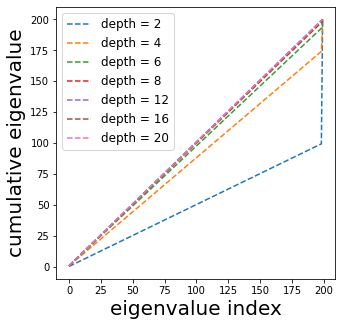
\includegraphics[scale=0.3]{figs/dgn-fra-ecdf-ideal-small.png}
\caption{Ideal spectrum of $\E{K_0}/d$ for a memorisation network for $n=200$.}
\label{fig:ideal-spectrum}
\end{figure}


\textbf{Why increasing depth till a point helps ?} 
We have:
%\comment{
\begin{align}\label{eq:mat}
\frac{\E{K_0}}{d}=\left[\begin{matrix}
1 &\mu^{d-1} &\ldots &\mu^{d-1} &\ldots\\ 
\ldots &1 &\ldots &\mu^{d-1} &\ldots\\ 
\ldots &\mu^{d-1} &\ldots &1 &\ldots \\
\ldots &\mu^{d-1} &\ldots &\mu^{d-1} &1\\ 
\end{matrix}\right]
\end{align}
%}
i.e., all the diagonal entries are $1$ and non-diagonal entries are $\mu^{d-1}$. Now, let $\rho_i\geq 0,i \in [n]$ be the eigenvalues of $\frac{\E{K_0}}{d}$, and let $\rho_{\max}$ and $\rho_{\min}$ be the largest and smallest eigenvalues.  One can easily show that $\rho_{\max}=1+(n-1)\mu^{d-1}$ and corresponds to the eigenvector with all entries as $1$, and $\rho_{\min}=(1-\mu^{d-1})$ repeats $(n-1)$ times,  which corresponds to eigenvectors given by $[0, 0, \ldots, \underbrace{1, -1}_{\text{$i$ and $i+1$}}, 0,0,\ldots, 0]^\top \in \R^n$ for $i=1,\ldots,n-1$. Note that as $d\ra\infty$, $\rho_{\max},\rho_{\min}\ra 1$.

\textbf{Why increasing depth beyond a point hurts?} 
In \Cref{th:mainrefined}, note that for a fixed width $w$, as the depth increases the variance of the entries $K_0(s,s')$ deviates from its expected value $\E{K_0(s,s')}$. Thus the structure of the Gram matrix degrades from \eqref{eq:mat}, leading to smaller eigenvalues.
\FloatBarrier
\begin{figure}[h]
\resizebox{\textwidth}{!}{
\begin{tabular}{cccc}
%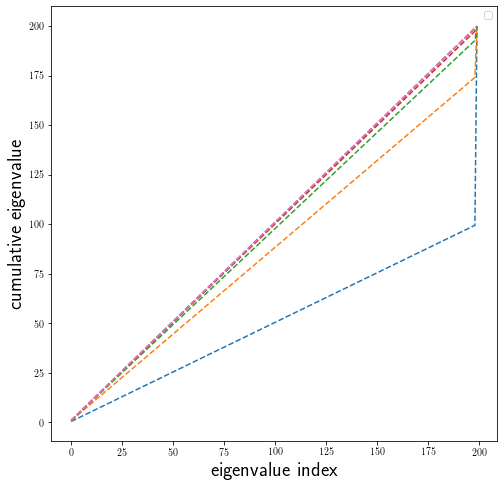
\includegraphics[scale=0.4]{figs/dgn-fra-ecdf-ideal.png}
%&
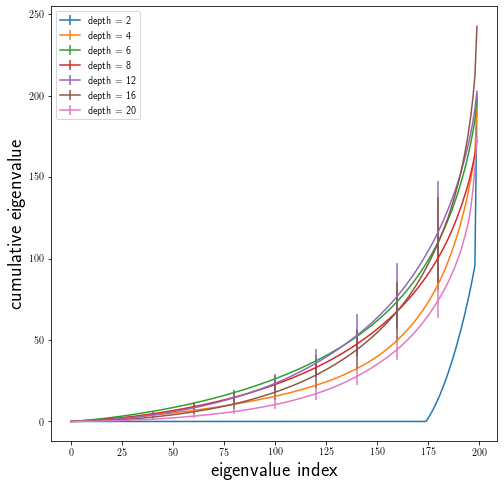
\includegraphics[scale=0.5]{figs/dgn-fra-ecdfbyd-w25.png}
&
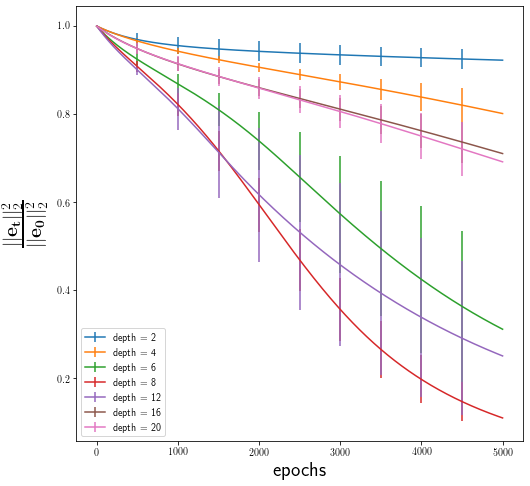
\includegraphics[scale=0.5]{figs/dgn-fra-conv-w25.png}
&
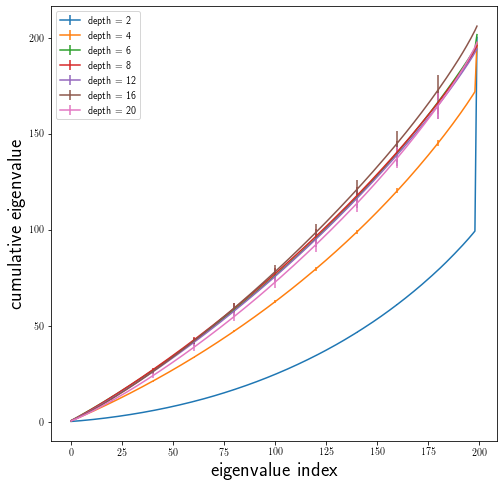
\includegraphics[scale=0.5]{figs/dgn-fra-ecdfbyd-w500.png}
&
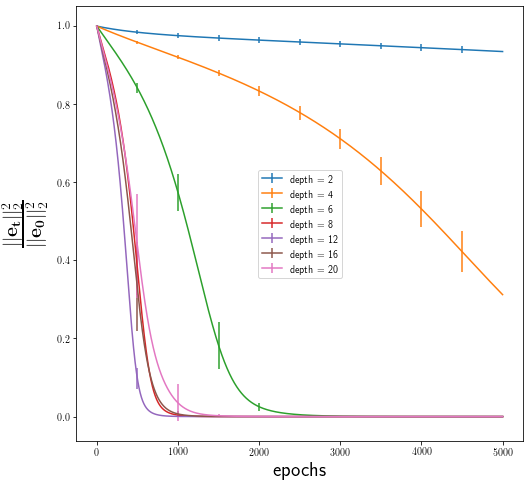
\includegraphics[scale=0.5]{figs/dgn-fra-conv-w500.png}
\end{tabular}
}
\caption{Shows the plots for the memorisation network with $\mu=\frac{1}{2}$ and $\sigma=\sqrt{\frac{2}{w}}$. The number of points to be memorised is $n=200$. The left most plot shows the e.c.d.f for $w=25$ and the second plot from the left shows the error dynamics during training for $w=25$. The second plot from the right shows the e.c.d.f for $w=500$ and the right most plot shows the error dynamics during training for $w=500$. All plots are averaged over $10$ runs.}
\label{fig:dgn-frg-gram-ecdf}
\end{figure}

\subsection{Experiment}
We set $n=200$, and $y_s\sim\text{Uniform}[-1,1]$. We look at the cumulative eigenvalue (e.c.d.f) obtained by first sorting the eigenvalues in ascending order then looking at their cumulative sum. The ideal behaviour (\Cref{fig:ideal-spectrum}) as predicted from theory is that for indices $k\in[n-1]$, the e.c.d.f should increase at a linear rate, i.e., the cumulative sum of the first $k$ indices is equal to $k(1-\mu^{d-1})$, and the difference between the last two indices is $1+(n-1)\mu^{d-1}$. In \Cref{fig:dgn-frg-gram-ecdf}, we plot the actual e.c.d.f for various depths $d=2,4,6,8,12,16,20$ and $w=25,500$ (first and third plots from the left in \Cref{fig:dgn-frg-gram-ecdf}). 

\textbf{Roles of depth and width:} In order to compare how the rate of convergence varies with the depth, we set the step-size $\alpha=\frac{0.1}{\rho_{\max}}$, $w=100$. We use the vanilla SGD-optimiser. Note the$ \frac{1}{\rho_{\max}}$ in the stepsize, ensures that the uniformity of maximum eigenvalue across all the instances, and the convergence should be limited by the smaller eigenvalues. We also look at the convergence rate of the ratio $\frac{\norm{e_t}^2_2}{\norm{e_0}^2_2}$. We notice that for $w=25$, increasing depth till $d=8$ improves the convergence, however increasing beyond $d=8$ worsens the convergence rate. For $w=500$, increasing the depth till $d=12$ improves convergence, and $d=16,20$ are worse than $d=12$.  %This matches with the depth phenomena observed in practical DNNs and also matches our theory.


\end{appendix}